\documentclass{llncs}
\usepackage{amsmath}
\usepackage{amssymb}
\usepackage{pgfplots}
\pgfplotsset{compat=1.8}
\usepackage{graphicx}
\usepackage[hidelinks]{hyperref}
\usepackage{multirow}
\usepackage{color}
%\usepackage{pifont}
\usepackage{bbding}
\usepackage{algorithm}
%\usepackage{algorithmic}
\usepackage{arevmath}     % For math symbols
\usepackage[noend]{algpseudocode}
\usepackage{multicol}
\usepackage{subfig}


\makeatletter
\newcommand{\rmnum}[1]{\romannumeral #1}
\newcommand{\Rmnum}[1]{\expandafter\@slowromancap\romannumeral #1@}
\makeatother


% to remove \sal, comment the 1st and de-comment the 2nd following lines:
\newcommand{\sal}[1]{\textcolor{red}{[\textbf{Sal:} #1]}}
%\newcommand{\sal}[1]{}


\begin{document}



\title{Path-Based Visual Explanation}

\author{Mohsen Pourvali\inst{1}}
\institute{Lenovo, China\\
\email{\{mpourvali\}@lenovo.com}
%\and
%Queensland University of Technology (QUT), Brisbane, Australia\\
%\email{mehrad.gharagozloo@qut.edu.au}
}

\maketitle


\begin{abstract}
Ability to explain behavior of a Machine Learning (ML) model as a black box to people is becoming an essential due to widely usage of ML applications in critical areas ranging from medicine to commerce. Case-Based Reasoning (CBR) received a special interest among other methods in providing explanation for model decision due to easily it can be paired with a black box and then proposes a post hoc explanation framework. In this paper, we propose a CBR-Based method to not only explain a model decision but also provide recommendations to the user in an easily understandable visual interface. Our evaluation of the method on three targeted users Artificial Intelligence (AI) novices, data experts, and AI experts show interesting results.
\end{abstract}

% A category with the (minimum) three required fields
%\category{H.3}{Information storage and retrieval}{Content Analysis and Ranking}

%\terms{Algorithms, Experimentation}

%\keywords{Keyphrase extraction, Text clustering} % NOT required for Proceedings

\section{Introduction}
Ability to explain behavior of a ML model to people is becoming an essential due to widely usage of ML applications in critical areas ranging from medicine to commerce. 

Most of the current explanation methods assign scores to input features, by which features that are important for model’s decisions are identified.
Explaining the underlying reasons for an image classification model’s decision to a human is easier than explaining a decision of text classification model. 

%It is more understandable for a human to be explained by showing him/her coherent pixels (i.e., segment) of the image as a reason of a model’s decision. 
%It is more understandable for a human to have a condensed-features visual imagery of a model decision than scattered-features explanation for a specific reason. Condensed-features means a collection of features side-by-side are exposed to human’s eyes that makes it easy to understand coherency of features in form of concepts, e.g., a segment of image, and better distinguishing the concepts.  
In image we can represent segments of the image as concepts \cite{ghorbani2019towards} which are understandable for human if we explain model's decision by using these concepts. For example, in an image of a girl her hair is a concept which is understandable for a AI novice if we explain to her this part of image was the main reason that model think this is a girl's picture. The understandable concepts in text could be a sentence or paragraph, like saying which sentence is the main reason for a model decision.
But, in tabular data, it is hard to explain reason of a model’s decision through the concepts. We define this difficulty as \textbf{Feature Inability} and \textbf{Feature Ambiguity} problems.

\subsubsection*{Feature Inability:}First problem is that, each feature in tabular data individually (like a single pixel in image) is not able to explain reason of the model’s decision, and also unlike what a collection of pixels in images as segments/super-pixel of image can do for understandability of an explanation, a collection of features in tabular data are not quite understandable by human since finding their internal relations is difficult.

\subsubsection*{Feature Ambiguity:}Another problem is that, meaning of a feature solely in tabular data might be ambiguous to a human like a single pixel in an image. But, unlike images in which a collection of coherent pixels makes it understandable for human, in tabular data even a collection of features still doesn't change ambiguity of the features. For instance, in an image of a dog, a single pixel is not meaningful, but it is possible to select a segment of pixel (e.g., dog’s leg) which is understandable for a human. In tabular data, features are like scattered pixels that even a collection of them possibly are not understandable to a human. 

A collection of coherent pixels as a segment of an image shows relations between the features/pixels in that segment which is understandable and meaningful to the human eyes. But, in tabular data even if there is relation between two features, it might be unclear to human. And this is because of the nature of images which comes from a real world object, all features already are defined and are put together, and there is an order that makes it easy to separate features in meaningful segments. Also, in text data, we can see this meaningful order and segmentation (e.g., sentence, paragraph) but not exactly like what exists in images. In tabular data, there is no meaningful order and segmentation in features.

Two above mentioned issues also indicate the importance of visualization of the explanation that enables user to interpret the underlying reasons for a model decision. 

A good explanation for a model prediction of an instance may not be a complete explanation of all the reasons, but in turn, it would be a contrastive explanation comparing what the differences were to another instance's prediction~\cite{molnar2020interpretable}.
Another factor for a good explanation could be providing a few recommendations to user. For example, if you apply for a loan and your application is rejected, you might want to not only know the reasons but also to understand the agent's reasoning in a bid to strengthen your next application~\cite{lipton2018mythos}.

We propose a Hybrid method to address these issues for any probability-based classification model. 
%Typically, an explanation algorithm entails three main components: a trained classification model, a set of test data from the same classification task, and an importance computation module that assigns importance to features. 
%In our proposed system, 
We first establish an explanation algorithm by taking advantage of Facts and Foils concepts. Considering explanations, people are not only interested in why event $P$ happened, they also want to know why not event $Q$ happened instead of event $P$. The event that did happen $P$ is referred to as Fact, and the contrast event that did not happen $Q$ is referred to as Foil~\cite{lipton2004inference}. %(adopting Lipton’s terminology).
A Foil could be any sample to be compared with a Fact, we consider the better samples and the best sample in a Path-Based fashion to compare with a Fact. Indeed, we try to address three questions from user as well, which are; why not a \textit{better} event, or why not the \textit{best} event happened, and an important question which is how to have/reach these events. We then present our Path-Based explanation with a visual interface which is easily understandable for a user.


\section{Related Works}
CBR enable us to present a post hoc mechanism to not only predict model result of a query case, but also explain model decision by using examples which are similar to the case with respect to the model. Indeed, CBR as a more interpretable system can be paired with a black box in a way that provides explanatory samples based on model prediction, in turn generate a \textit{twin-system}~\cite{keane2019case}. Authors in~\cite{keane2019case} survey similar approaches that use CBR in a post hoc fashion as one particular solution to the XAI problem. For example,~\cite{caruana1999case} uses a learned model as distance metric to find explanatory cases for an Artificial Neural Network (ANN) in medical domain. Authors use Euclidean distance to measure similarity between latent features (i.e., hidden units activation vector of ANN model) of the case to be explained and all the training dataset, and then they present cases with small Euclidean distance as the similar cases to the query case to then explain the ANN reasoning for the query case. In~\cite{nugent2005case}, authors select explanatory cases based on their similarity in their local important features to the query case to be explained.~\cite{cunningham2003evaluation} evaluate the usefulness of CBR in term of retrieve explanatory cases to explain prediction, and show that it is more convincing than one based on rules. 
\textcolor{red}{TODO}
Visualization of CBR-paired systems can even enhance understandability of the proposed explanation. \cite{massie2004visualisation} show that \textcolor{red}{here...}
\cite{lamy2019explainable} proposes a CBR system able to classify a query case using an automatic algorithm, but also through visual reasoning. Authors in \cite{lamy2019explainable} select similar cases in the feature/input space.

This work is inspired by \cite{lamy2019explainable},
Our approach in this context is a post-hoc approach to explain underlying reasons for a model decision, in which similar points are selected in the model result/output space, in our approach the samples sit next to each other for an specific goal which is to build a path from the query case to the best case in each class. these samples are selected from the candidate cases that their model results are close to a direct line in model output space drawn between query case result and the best case. We only use three colors in the visual interface, which makes it easier for user to identify dominant color. It also can be modified for blind people by using different shapes for each color. Providing a path from model output of a query case to the best result of the model can depict an \textbf{evolution} process, in turn can help user to understand how (s)he can get a better result from the model, furthermore, it can provide \textbf{recommendations} for this aim.

\section{Our Proposed Method}
Providing a path from a sample case as result of model to the best result of the model can depict an evolutionary process, in turn can help user to understand how (s)he can get a better result from the model. 
Furthermore, a path on which there are several cases from other classes implies a form of analogical reasoning: Case-Based Reasoning (CBR) in which the solution for a new case is determined using a database of previous known cases with their solutions.
Cases similar to the new case are retrieved from the database, and then their solutions are adapted to the case. 
This situation provides an Interpretable Classification, in which user can classify the new case according to his own knowledge and the knowledge retrieved from CBR. The proposed visual interface aims at identifying what is the dominant color? This approach can be either a proof for ML model decision, or in turn it helps user decide about which class query case belongs to. Focusing on explaining this differences results to the concept of recommendation, which represents some possible way by which we could had a different Fact.

A path from a query case to the best case of each class in the model result space provide a better understanding of the model due to evaluation of the similar cases appeared on the path. The visual interface included with a path that constructs CBR in ML results space provides a transparent insight of the ML, which can be used also to evaluate different ML models. Each specific model has its own Best case, Path, and similar cases on the path. 

Assuming a classification model with four classes $C_{1}$, $C_{2}$, $C_{3}$, $C_{4}$, and a result of the model E, our explanation algorithm selects two classes as default, the class of the query case result and the class with the highest probability, selecting classes can be also based on the user desire, and then it generates two paths each one from $E$ to a point $M_{i}$ that has the highest probability in that class. A path is generated by connecting a collection of points in the probability space that are very close to the direct line connecting $E$ to $M_{i}$ in 3-Dimension space.

In general, the workflow of the approach is two-step, in the first step, a 3-Dim model results space generated and two paths with similar cases are indicated, in the second step, a visual explanation for input case are generated.

\subsubsection*{First Step:} Given a vector $E=[e_{0},e_{1},e_{2},...,e_{N-1}]$ with $N$ dimensions as a distribution over $N$ classes for a classification model with an input case, (a) two classes $C_{1}$ and $C_{2}$ based on user desire or default classes are selected, (b) rest of the classes' probabilities are reduced to one dimension to generate a new vector $E'=[e_{1},e_{2},e_{rest}]$, (c) from each class, the best sample is selected which is a result of the model for a sample that has highest probability in corresponding dimension of its distribution. 
%(d) Dimensions of all the distributions in the model result space are reduced to 3-Dim (dimensions of the two desired classes remain as before and summation of other dimensions as third dimension), 
(d) two paths from $E'$ to $C_{1}$ and $C_{2}$ are conducted by which close cases to the path are identified as Explanatory Cases (EC), Figure~\ref{fig:path}. In order to depict the evolution process for the sample case $E'$, each path is divided into several areas, and from each area an EC is selected. Indeed, these ECs build our paths through which we can see how features of a sample case are changed to reach the best result in each class. Each EC is a case from corresponding class for which result of the model is close to the direct line/path between $E'$ and the best result in that class. Indeed, the path is a direct line in 3-Dim between model result of the query case and the best case, and ECs are the closest point in model result space to this line. 
%The ECs are those in model's result space which are close to the direct line between the query case and the bets case, 
The distance between point (model's results) and direct line (path) is calculated using following formula:

\begin{equation}
d_{i} = \frac{\left| \overline{p_{i}E} \times \overline{s} \right|}{\left|\overline{s}\right|}
\end{equation}

\noindent where $p_{i}=[p_{i0},p_{i1},p_{i2}]$ is candidate similar case, $E$ is the query case, and $s=[(e_{0}-p_{i0}),(e_{1}-p_{i1}),(e_{2}-p_{i2})]$ is directing vector of the line.

\textcolor{red}{The algorithm for recording the suggestions is shown in Algorithm 1.}

\begin{algorithm}
	\caption{Algorithm for recording the suggestions}
	\begin{algorithmic}
		\begin{small}
			\Function{SuggRecord}{$p_{i}$}
			\State $Comb\_Feat = \{feat | feat.Value \notin G \}$ 
			\If{condition}
			\EndIf
			\EndFunction
		\end{small}
		
	\end{algorithmic}
\end{algorithm}


\begin{figure}
	\centering
	
	\subfloat[\centering The paths to the best cases in class $C_{1}$ and class $C_{2}$]{
		\label{fig:path}
		\def\svgwidth{150pt}
		\input{path.pdf_tex}
	}
    \qquad
    \subfloat[\centering various space size of Explanatoty Samples]{
    	\label{fig:samp}
    	\def\svgwidth{150pt}
    	\input{samplespace.pdf_tex}
    }
    
	\caption{2-Dim Visual illustration of paths and explanatory samples space.}
\end{figure}

\subsubsection*{Second Step:} In the second step, we generate a Visual Explanation as shown in \textcolor{red}{Figure 2}, which is inspired by Rainbow Boxes \cite{lamy2017rainbow}. As it is shown in Figure 2, corresponding model's input case query for vector $E'$ is in the middle of the explanation, the best case for each class is located at each corner. The classes at the corners of the explanation are two classes based on user desire or default classes.

Characteristics of the Visual Explanation is as follows: 
\begin{itemize}
	\item The ECs on each path identified by different colors corresponding to the closeness of their 3-Dim distribution result in scatter plot to the query case shown in Figure 1.
	\item The value inside each box is the feature value, thus, user is able to explore the feature's change through each path to the best result of the model.
	\item The column width of similar cases is proportional to the distance between similar case and the path (i.e., the line that connects query case to the best case), farther cases are shown by smaller column width.
	\item As it can be seen in Figure 2, the length of each box is different, indeed, they are proportional to the importance of the corresponding feature (feature score) for that box. For example, feature number 1 is the most important feature. To rank feature importance we use LIME with the aim of finding a local feature importance for query case. 
	\item Blue color shows that the sample case is closer to Low class and result of the model is also Low, but user might think of more important features shared between the Query case and Similar Cases from class High. 
\end{itemize}
 
Therefore, this explanation of a case in tabular data can address two above problems: Feature Inability, using Case-Based Reasoning with cases which are considered to be better than query case provides an understandable view of explanation for user, by collection of connected features-being in a same path; Feature Ambiguity, a path that explains the process of feature’s value change to enhance probability of being selected as a better member of a class (in model point of view) build a coalition of cases with similar or different feature’s value- all aims in one goal that can help in disambiguating of the feature and relations between them.
A general overview of my proposal is shown in Figure 3.  

In Figure 3, you can recognize at a glance that class Low is a better choice to classify query case in it, considering dominant Blue color. Furthermore, we can see more information in Figure 3 like suggestion which means representing information by which we can get better result from the model. For example, if we walk in the path of class No, we would get better result for query case, if we only replace value of feature RprTp by software instead of rur. In the other word, if we want to have better result of the model, going one step toward the best result of the model in class High, and also are allowed to only change one feature’s value, then, feature RprTo would be one of the best features and for which value software is one the best value to choose. We identify these information by
replacing feature's values of the query with the feature's values of the specific sample on the path. The goal is to minimize the distance between the model result of the query and specific sample on the path. Indeed, similar to Shapley value calculation, we try to find feature's value has the highest contribution to increase probability of the query case in a class.
, in which there is only one sample (i.e., the sample in the step that we want to get there), and a coalition with only one member (we can increase number of members in the coalition). 

Another information that we can acquire in Figure 3 is priority of the feature's value, on the path to the best sample in class No it is shown that from sample 1 to sample 6 the best feature to its value be replaced with query case is RprTp, but about last sample which is the best sample also, the best feature becomes fRetCount. Indeed, for the sample 6 and the best sample, all the important features have the same values which is expected to still value of feature RprTp be the best choice to be replaced with rur, but as it is shown fRetCount is better, the value for fRetCount in all the samples except last one is 1. Considering two last samples which are same in most important features, it shows that value 305 for feature fRetCount has the higher impact in class No compared to value hardware with parts for feature RprTp.
 
\section{Visual Interface}


\begin{figure}	
	\centering
	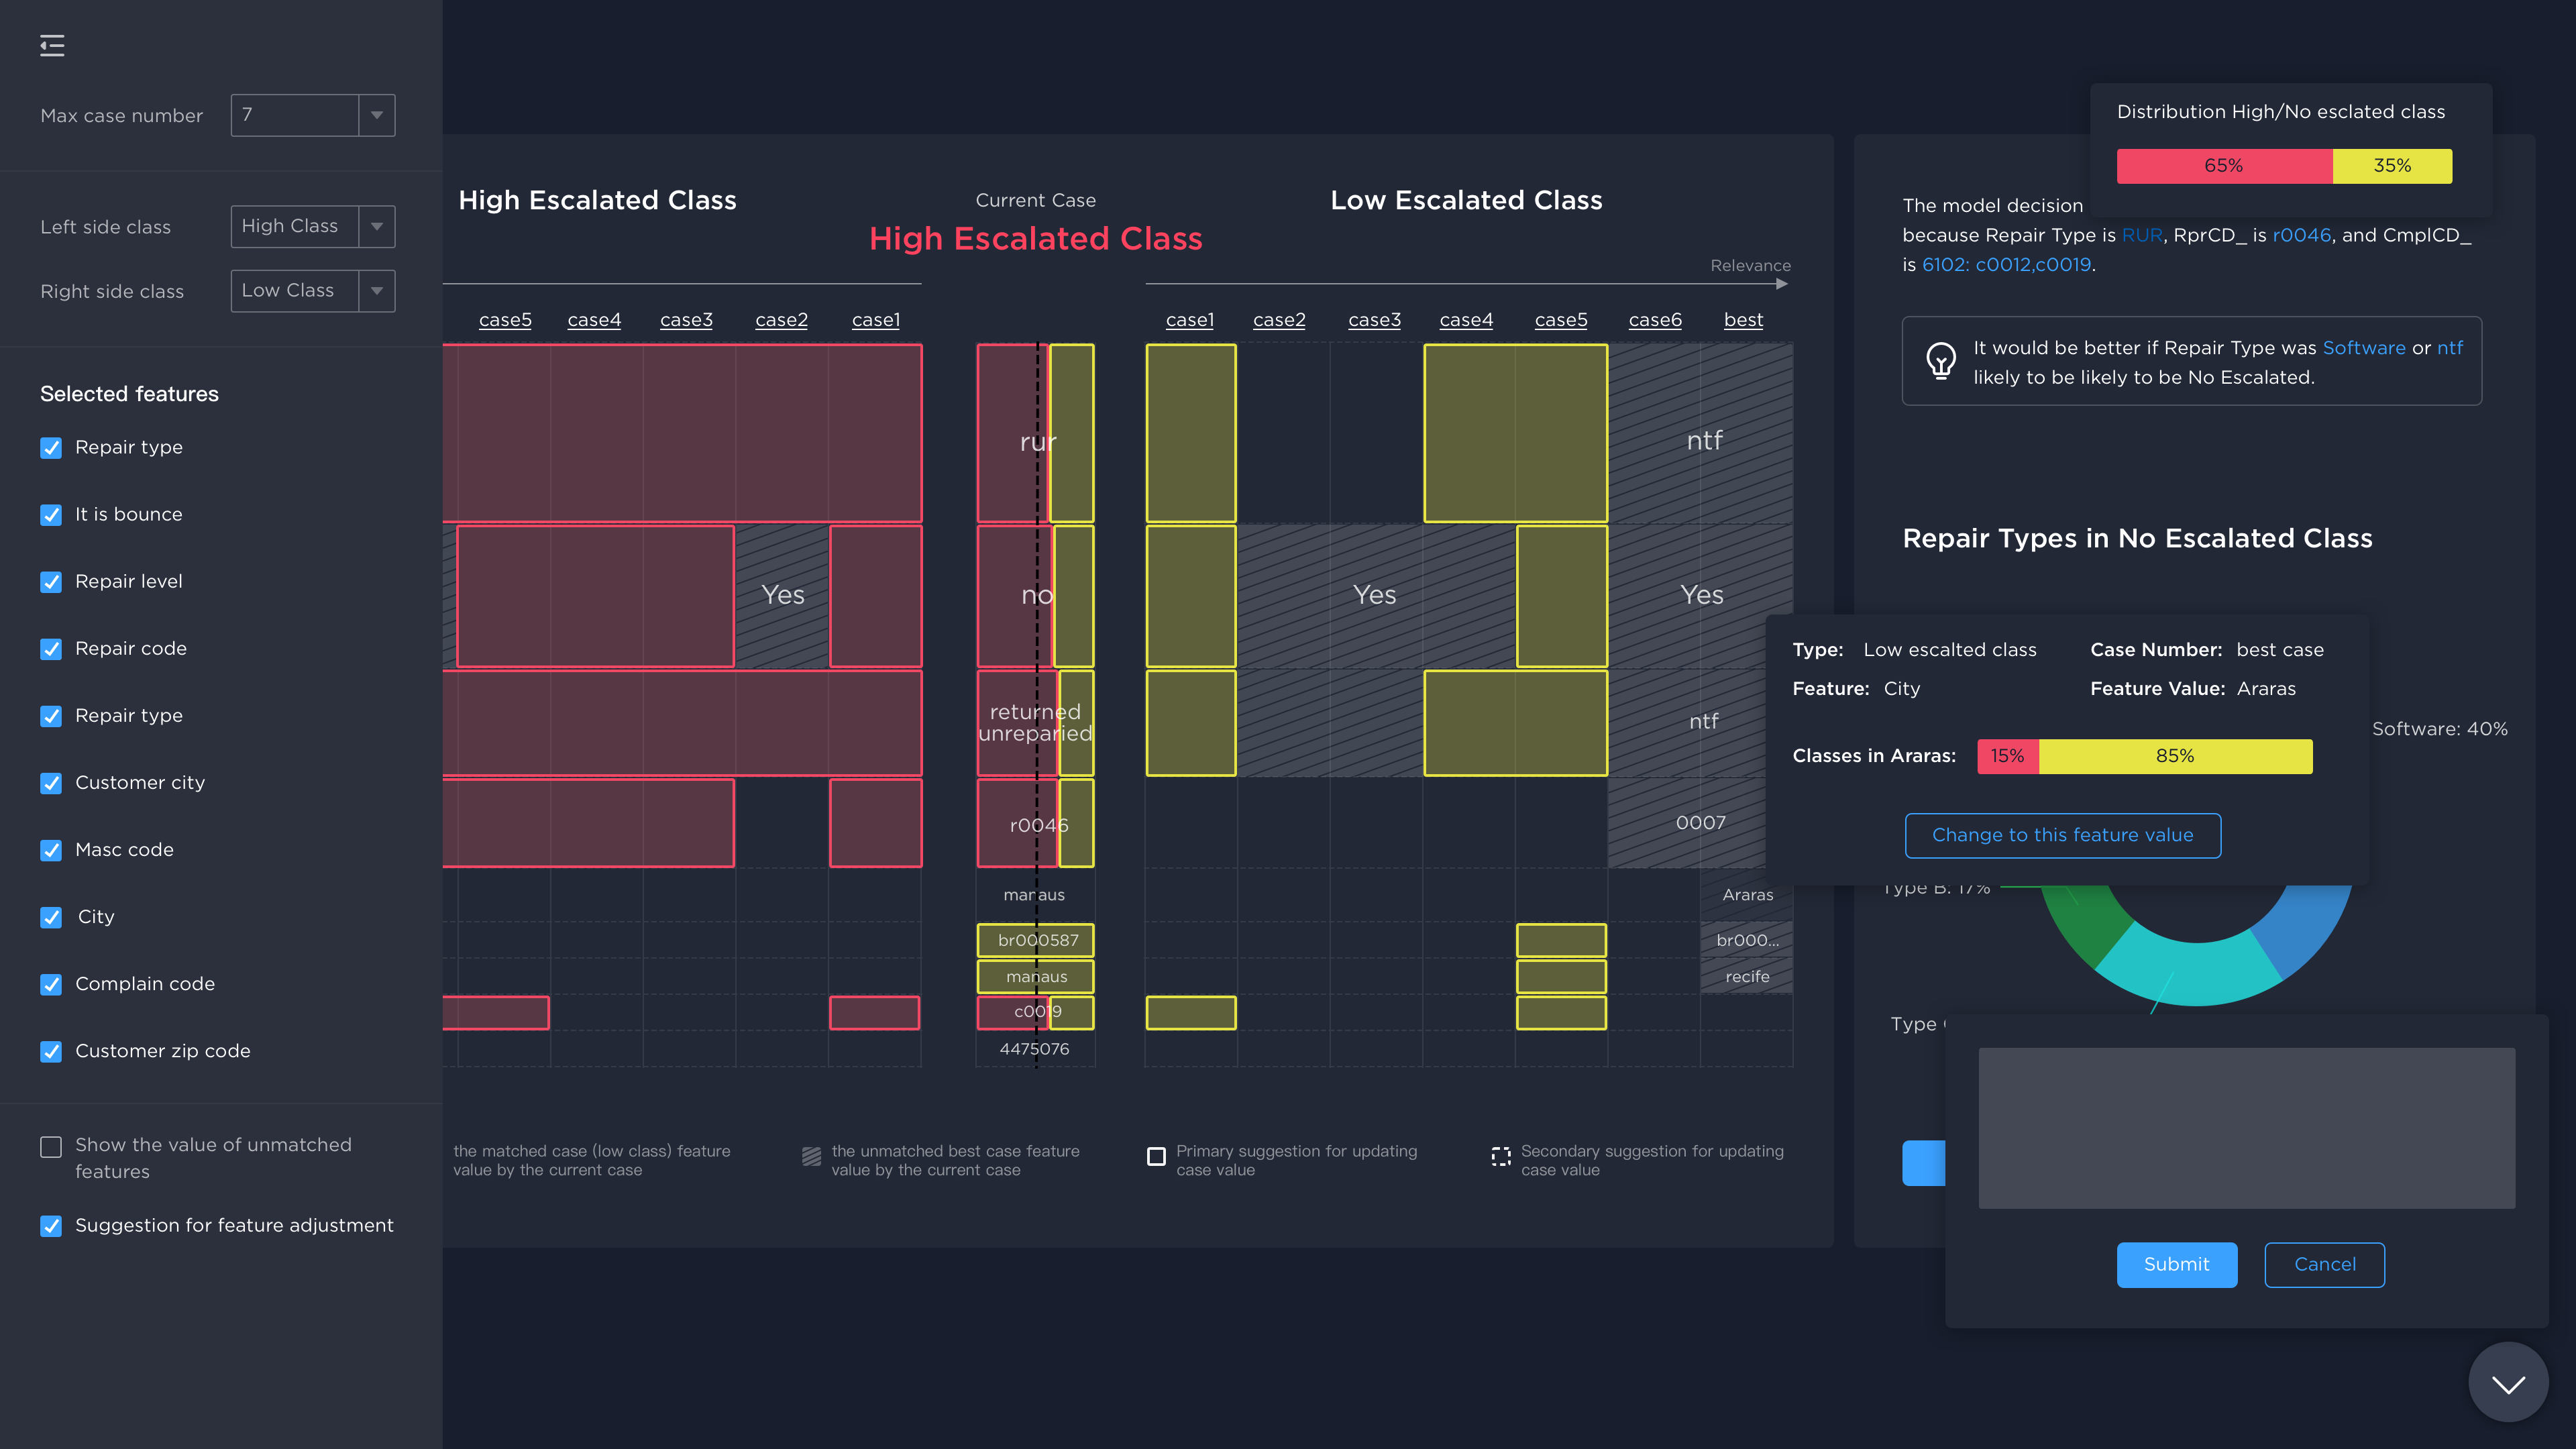
\includegraphics[scale=0.1]{1_3_xai.png}
	\centering\caption{A snapshot of the interface}	
\end{figure}


 
\section{Experimental Setup}
\textcolor{red}{TODO} We compare our visual explanation in two ways; in the first comparison, we generate a natural language-based explanation using feature importance from LIME and a Supporting Statistics extracted from seen/unseen data.

In the second comparison, we compare our visual explanation with the proposed method in 
\subsection{Datasets}


\subsubsection{Preprocessing}

\subsection{Baselines}

\subsection{Evaluation Measures}

\section{Experimental Results}

\section{Conclusion}

This is conclusion..

This is our future work..

%\section{References}

\bibliographystyle{abbrv}
\bibliography{Bibliography}


\end{document}
